\documentclass[a4paper,twoside,BCOR=20mm]{scrreprt}
\usepackage[utf8]{inputenc}
\usepackage[T1]{fontenc}
\usepackage[ngerman]{babel}	% german hyphenation, quotes, etc
\usepackage[ngerman]{translator}
\usepackage{amsmath}
\usepackage{paralist}
\usepackage{amsfonts}
\usepackage{acronym}
\usepackage{enumerate}
\usepackage{hyperref}
\usepackage{amssymb}
\usepackage{caption}
\usepackage{multirow}
\usepackage{graphicx}
\usepackage{tabularx}
\usepackage{color}
\usepackage{wrapfig} % wrap text around figures
\usepackage{subfig} % align two pics beside each other
\usepackage[table,xcdraw]{xcolor}
\hypersetup{ 					% ‘texdoc hyperref‘ for options
	pdftitle={PSE PCC: Designentwurf},
	pdfauthor={Giorgio Groß, Christoph Hörtnagl, David Laubenstein,  Josh Romanowski,  Fabian Wenzel},
	bookmarks=true,
}
\title{Designentwurf: Privacy Crash- Cam}

%Paket laden
\usepackage[
numberedsection,
nonumberlist, %keine Seitenzahlen anzeigen
acronym,      %ein Abkürzungsverzeichnis erstellen
toc,          %Einträge im Inhaltsverzeichnis
section]      %im Inhaltsverzeichnis auf section-Ebene erscheinen
{glossaries}

%Befehle für Abkürzungen
\newacronym{KIT}{KIT}{Karlsruher Institut für Technologie}

%Richtige Silbentrennungen
\hyphenation{Ein-stel-lun-gen}

% KIT layout

\definecolor{orange}{rgb}{1,0.5,0}
\definecolor{mintgreen}{RGB}{50,161,137}
\definecolor{gray}{RGB}{120,120,120}

\usepackage[color]{changebar}
\cbcolor{gray}
\changebarwidth 0.5pt

\usepackage{fancyhdr}
\pagestyle{fancy}
 \fancyhf{} %alle Kopf- und Fußzeilenfelder bereinigen 
 
 \fancypagestyle{plain}{} %Kopf- und Fußzeile auf jeder Seite	 
	\fancyhead[L]{PCC-Designentwurf}
	\fancyhead[R]{\leftmark}
	\rhead{\nouppercase{\leftmark}}
	\renewcommand{\headrulewidth}{0.5pt}
	\renewcommand{\headrule}{\hbox to\headwidth{%
		\color{mintgreen}\leaders\hrule height \headrulewidth\hfill}}

\raggedbottom

	\renewcommand{\footrulewidth}{0.5pt}
	\renewcommand{\footrule}{\hbox to\headwidth{%
  		\color{mintgreen}\leaders\hrule height \headrulewidth\hfill}}				
	\fancyfoot[LE,RO]{\thepage}


\setcounter{tocdepth}{5}
\makeglossaries
\begin{document}
\begin{titlepage}

\begin{center}


\includegraphics[width=0.5\linewidth]{Res/KITLogo.png}\\[0.5cm]
  

\textsc{\bfseries Fraunhofer Institut für Optronik, Systemtechnik und Bildauswertung}\\[0.5cm]
\textsc{Mario Kaufmann\\Pascal Birnstill\\Erik Krempel}\\[2cm]

\textsc{\LARGE \bfseries Designentwurf}\\[0.5cm]
\textsc{\bfseries Version 0.1}\\[0.2cm]


\newcommand{\HRule}{\rule{\linewidth}{0.5mm}} 
{\color{mintgreen}\HRule} \\[0.4cm]
{\huge \bfseries Privacy Crash Cam App für Android}\\[0.4cm]
{\color{mintgreen}\HRule} \\[1cm]

% \textsc{\Large \bfseries Gruppe :}\\[0.3cm] 
\textsc{\Large Fabian Wenzel\\ Giorgio Groß\\ Christoph Hörtnagl\\ David Laubenstein\\[0.15cm]Josh Romanowski} \\[2cm]

{\large \today}

\end{center}

\end{titlepage}
% \maketitle
\tableofcontents
\newpage
%content

% PUT GENERAL (INTRODUCTION ...) CONTENT HERE
\chapter{Architektur}
\section{Model View Presenter (MVP)}
Beim Design der Privacy Crash Cam wird schnell deutlich, dass eine strikte Trennung zwischen Datenbank, Applikationslogik und Benutzeroberfläche von Vorteil ist. Neben einer übersichtlichen Unterteilung in einzelne Module unterstützt dieses Vorgehen die Austauschbarkeit der einzelnen Module, deren Wiederverwendbarkeit und Plattformunabhängigkeit. Das Model-View-Presenter-Prinzip realisiert diese Trennung und wird auf auf App und Web interface übertragen.\linebreak\par

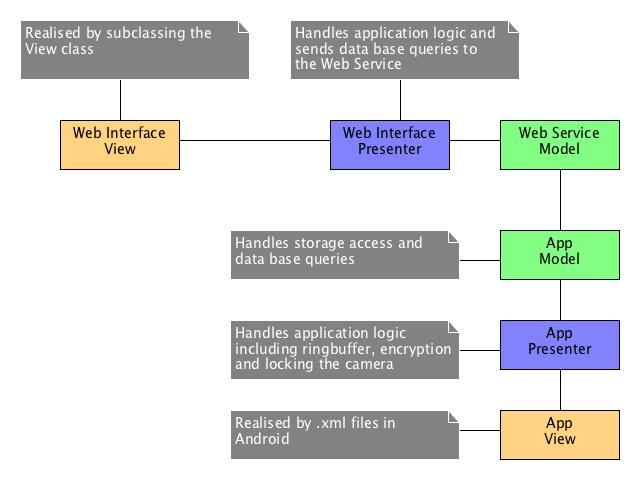
\includegraphics[scale=0.5]{./resources/Diagramme/overview_mvp.jpg}

Die Model-Rolle wird vom Web-Dienst erfüllt. Dieser bietet eine REST API, die sowohl vom Web Interface als auch von der App per HTTP-Anfragen angesprochen wird. Falls weitere Software entwickelt wird, mit der auf die Datenbank zugeriffen werden soll, soll diese ebenfalls auf die selbe API zugrifen können.\linebreak
Darüber hanus besitzt die App ein zusätzliches Model-Modul, das den Speicherzugriff regelt.\linebreak\par

Die Apllikationslogik wird durch die Presenter-Ebene umgesetzt. Hierbei besitzen App und Web Interface eigene Presenter-Module, die an die jeweilige Plattform angepasst sind. Der Presenter handhabt Eingaben durch Nutzer oder Sensoren und koordiniert die darauf folgenden Aktionen, wie das Ändern der Ansicht, Aktualisieren der Ansichten und den Zugriff auf die Model Ebene.\linebreak\par 

Die Rolle der View übernimmt schließlich die GUI. In Android wird diese durch entsprechende XML Dokumente implementiert, in Vaadin durch spezielle Java Klassen die von der Vaadin-Internen Klasse ``UI'' erben. Instanzierung, Manipulation und Navigation erfolgen schließlich durch die Presenter-Ebene, die Bindung erfolgt durch Beobachter und ist bereits durch das jewilige Framework festgelegt.



% PUT APP CONTENT HERE
\chapter{App}

\section{Modulübersicht}
\subsection{Presenter}
\section{Klassenübersicht}

\subsection{Presenter-Modul}
\subsubsection{CameraActivity} \label{app:klasse:CameraActivity}
\textbf{extends} \nameref{app:klasse:MainActivity} \newline
Die CameraActivity zeigt die CameraView an, instanzert eine CompatCameraHandler Instanz sowie eine IRecordCallback Instanz und manipuliert die graphische Nutzeroberfläche abhängig von den Methoden, die auf der IRecordCallback Instanz aufgerufen werden. Nach dem Start blendet die CameraActivity ein Symbol ein, welches die Bereitschaft der App signalisisert. Die CameraActivity stellt einen Observer des CompatCameraHandler dar.
\newline

\underline{Attribute}
\begin{itemize}
\itemsep0pt

\item \textbf{statusSymbol: ImageView} \hfill\\ 
\textbf{Sichtbarkeit} private\newline
ImageView die verwendet wird, um das Symbol einzublenden, welches die Bereitschaft bzw. die Aufnahme der App signalisiert.

\item \textbf{recordCallback: \nameref{app:klasse:IRecordCallback}} \hfill\\ 
\textbf{Sichtbarkeit} private\newline
Implementiert das IRecordCallback Interface. 
Der Aufruf der Mehtode \textit{onRecordStarted} benachrichtigt die CameraActivity Instanz über den Start der Videoaufnahme. Sie blendet das Symbol ein, welches die Aufnahme signalisiert. Das Symbol, welches zuvor die Bereitschaft der App signalisiert hat, wird ausgeblendet.
Der Aufruf der Methode \textit{onRecordStopped} benachrichtigt die CameraActivity Instanz über das Ende der Videoaufnahme. Sie blendet das Symbol ein, welches die Bereitschaft signalisiert. Das Symbol, welches zuvor die Aufnahme der App signalisiert hat, wird ausgeblendet.

\item \textbf{cameraHandler: \nameref{app:klasse:CompatCameraDataHandler}} \hfill\\ 
\textbf{Sichtbarkeit} private\newline
CameraHandler Instanz, die die Vorschaubilder der Kamera eigenständig verarbeitet und die Aufnahme auslößt. Diesem Feld wird eine TriggeringCompatCameraHandler Instanz zugewiesen.

\item \textbf{cameraView: \nameref{app:klasse:CameraView}} \hfill\\ 
\textbf{Sichtbarkeit} private\newline
CameraView Instanz, welche verwendet wird, um die Kameravorschau anzuzeigen.

\end{itemize}

\underline{Konstruktoren}\newline
\indent Keine, da der Lebenszyklus dieser Klasse von Android gesteuert wird.\newline

\underline{Methoden}
\begin{itemize}
\itemsep0pt

\item \textbf{Launch (callingActivity: Activity): void}\hfill\\
\textbf{Sichtbarkeit} public\newline
Startet ein neues Intent durch welches eine CameraActivity Instanz erzeugt und gestartet wird.

\item \textbf{getLayoutRes (): int}\hfill\\
\textbf{Sichtbarkeit} public\newline
Überschreibt die \textit{getLayoutRes} Methode der Superklasse.

\item \textbf{onCreate (savedInstanceState: Bundle): void}\hfill\\
\textbf{Sichtbarkeit} public\newline
Überschreibt die \textit{onCreate} Methode der Superklasse. Lädt die CameraView Instanz und erstellt die IRecorderCallback und CompatCameraHandler Instanzen.

\item \textbf{onResume (): void}\hfill\\
\textbf{Sichtbarkeit} public\newline
Überschreibt die \textit{onResume} Methode der Superklasse. Ruft die Methode \textit{setVisibility} der CameraView Instanz auf und übergibt den Parameter \textit{View.VISIBLE}.

\item \textbf{onPause (): void}\hfill\\
\textbf{Sichtbarkeit} public\newline
Überschreibt die \textit{onPause} Methode der Superklasse. Ruft die Methode \textit{setVisibility} der CameraView Instanz auf und übergibt den Parameter \textit{View.VISIBLE}.

\end{itemize}

\subsection{CameraLogic-Modul}

\subsection{MemoryAcess-Modul}

\subsection{ServerAcess-Modul}

\subsection{Utils-Modul}

% PUT WEB SERVICE CONTENT HERE


% PUT WEB INTERFACE CONTENT HERE
\section{Webinterface}
Das Webinterface Modul dient zur Bedienung des Webinterface. Dieses Modul enthält alle Klassen die zur Funktionalität des Webinterface beitragen. In diesem Modul wurde nach der Model-Präsentator-Anzeige Architektur entworfen. Wobei das Model hier mehr ein Stellvertreter von unserem tatsächlichen Model, dem Web-Dienst, ist. Dieser Stellvertreter übernimmt dann die Kommunikation mit dem Web-Dienst. Den Präsentator bilden die Klassen, Navigator und die Daten Manager. Navigator ist verantwortlich für das wechseln der Ansicht und die Daten Manager, sorgen dafür, dass die Daten in ihren Anzeige Objekten angezeigt werden können. Zuletzt die Anzeige, besteht aus verschiedenen Ansichten und einem Menü, in welchem zwischen den Ansichten gewechselt werden kann. Herzstück ist die Klasse UI, die für die Initialisierung verantwortlich ist und Navigator und das Menü hält.
\newpage
\newpage
\subsection{UI extends UI(com.vaadin.ui.UI)}
Die UI Klasse bildet das Herzstück des Webinterface. Die init[VERLINKEN] Methode dieser Klasse wird beim öffnen des Webinterface aufgerufen. Diese Klasse hat die Aufgabe alle Komponenten zu initialisieren und bildet dazu die Grundlage für alle graphischen Einheiten. Irgendwas zu Servlet sollte hier noch gesagt werden.
\begin{itemize}
\item \subsubsection{Attribute}
\begin{itemize}
\item \textbf{background VerticalLayout(com.vaadin.ui.VerticalLayout)} \hfill\\ 
Der background ist die Grundlage der graphischen Oberfläche des Webinterface. Darauf werden dann die Komponenten für das Menü und für die Ansichten gelegt. Dieses Attribut wird in der init[VERLINKEN] Methode erzeugt und initialisiert.

\item \textbf{menuArea VerticalLayout (com.vaadin.ui.VerticalLayout)} \hfill\\ 
Die menuArea ist die Grundlage für das Menü, in diesen Bereich wird das Menü gelegt. Dieses Attribut wird in der init[VERLINKEN] Methode erzeugt und initialisiert.

\item \textbf{contentArea VerticalLayout (com.vaadin.ui.UI)} \hfill\\ 
Die contentArea ist die Grundlage für die Ansichten, in diesen Bereich werden die Ansichten gelegt. Dieses Attribut wird in der init[VERLINKEN] Methode erzeugt und initialisiert.

\item \textbf{menu Menu (com.NOCHFESTLEGEN)} \hfill\\ 
Das menu bildet die Steuereinheit für den Benutzer. Durch das menu kann der Benutzer zwischen den verschiedenen Ansichten wechseln. Der Navigator wird in der init[VERLINKEN] Methode erzeugt und initialisiert.

\item \textbf{navigator Navigator (com.vaadin.navigator.Navigator)} \hfill\\ 
Der Navigator hat die Aufgabe, zwischen den verschiedenen Ansichten des Webinterface zu wechseln und diese in die contentArea zu laden. Der Navigator wird in der init[VERLINKEN] Methode erzeugt und initialisiert.

\end{itemize}

\item \subsubsection{Methoden}
\begin{itemize}
\item \textbf{init(VaadinRequest request} \hfill\\ 
Eingabeparameter: request

Ausgabeparameter:

In dieser Methode wird zuerst die Grundlage für die graphische Oberfläche erzeugt. Dann werden alle graphischen Komponenten, der navigator und das menu erzeugt und initialisiert. Am Schluss wird noch das menu gesetzt und die LoginView angezeigt.

\end{itemize}

\end{itemize}
%\newpage
%\input{./subtopicsDesign/Klassen/WebInterface/Klasse2}
%\newpage
%\input{./subtopicsDesign/Klassen/WebInterface/Klasse3}

\chapter{Anhang}

\section{Sequenzdiagramme}

\begin{figure}[ht]
	\centering
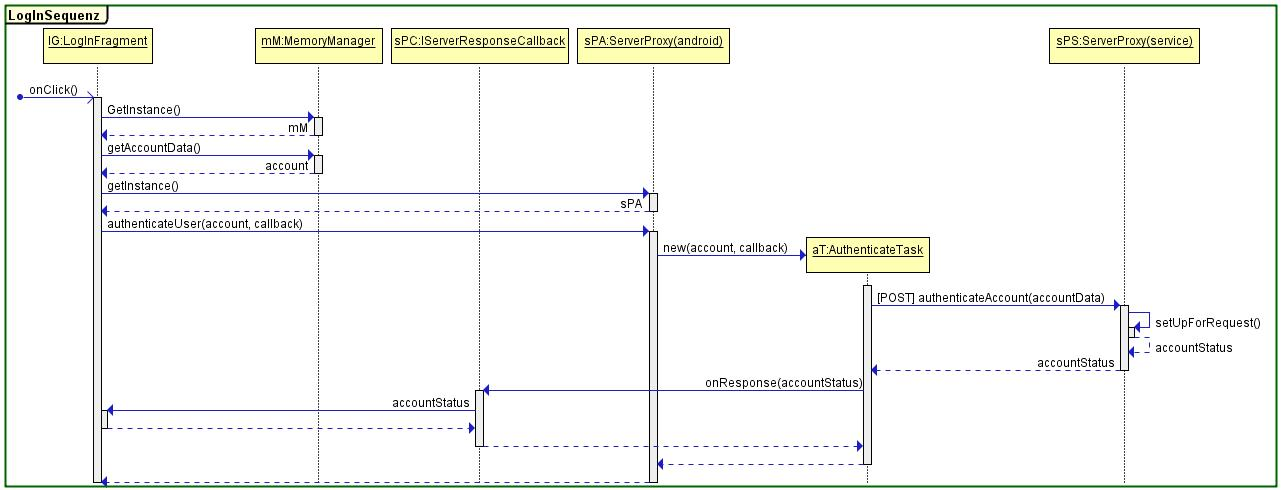
\includegraphics[width=1\textwidth]{./resources/Diagramme/App/logInSequence.jpg}
\caption{Anmelden in der App}
	\label{fig:AppAuth}
\end{figure}

\begin{figure}[ht]
	\centering
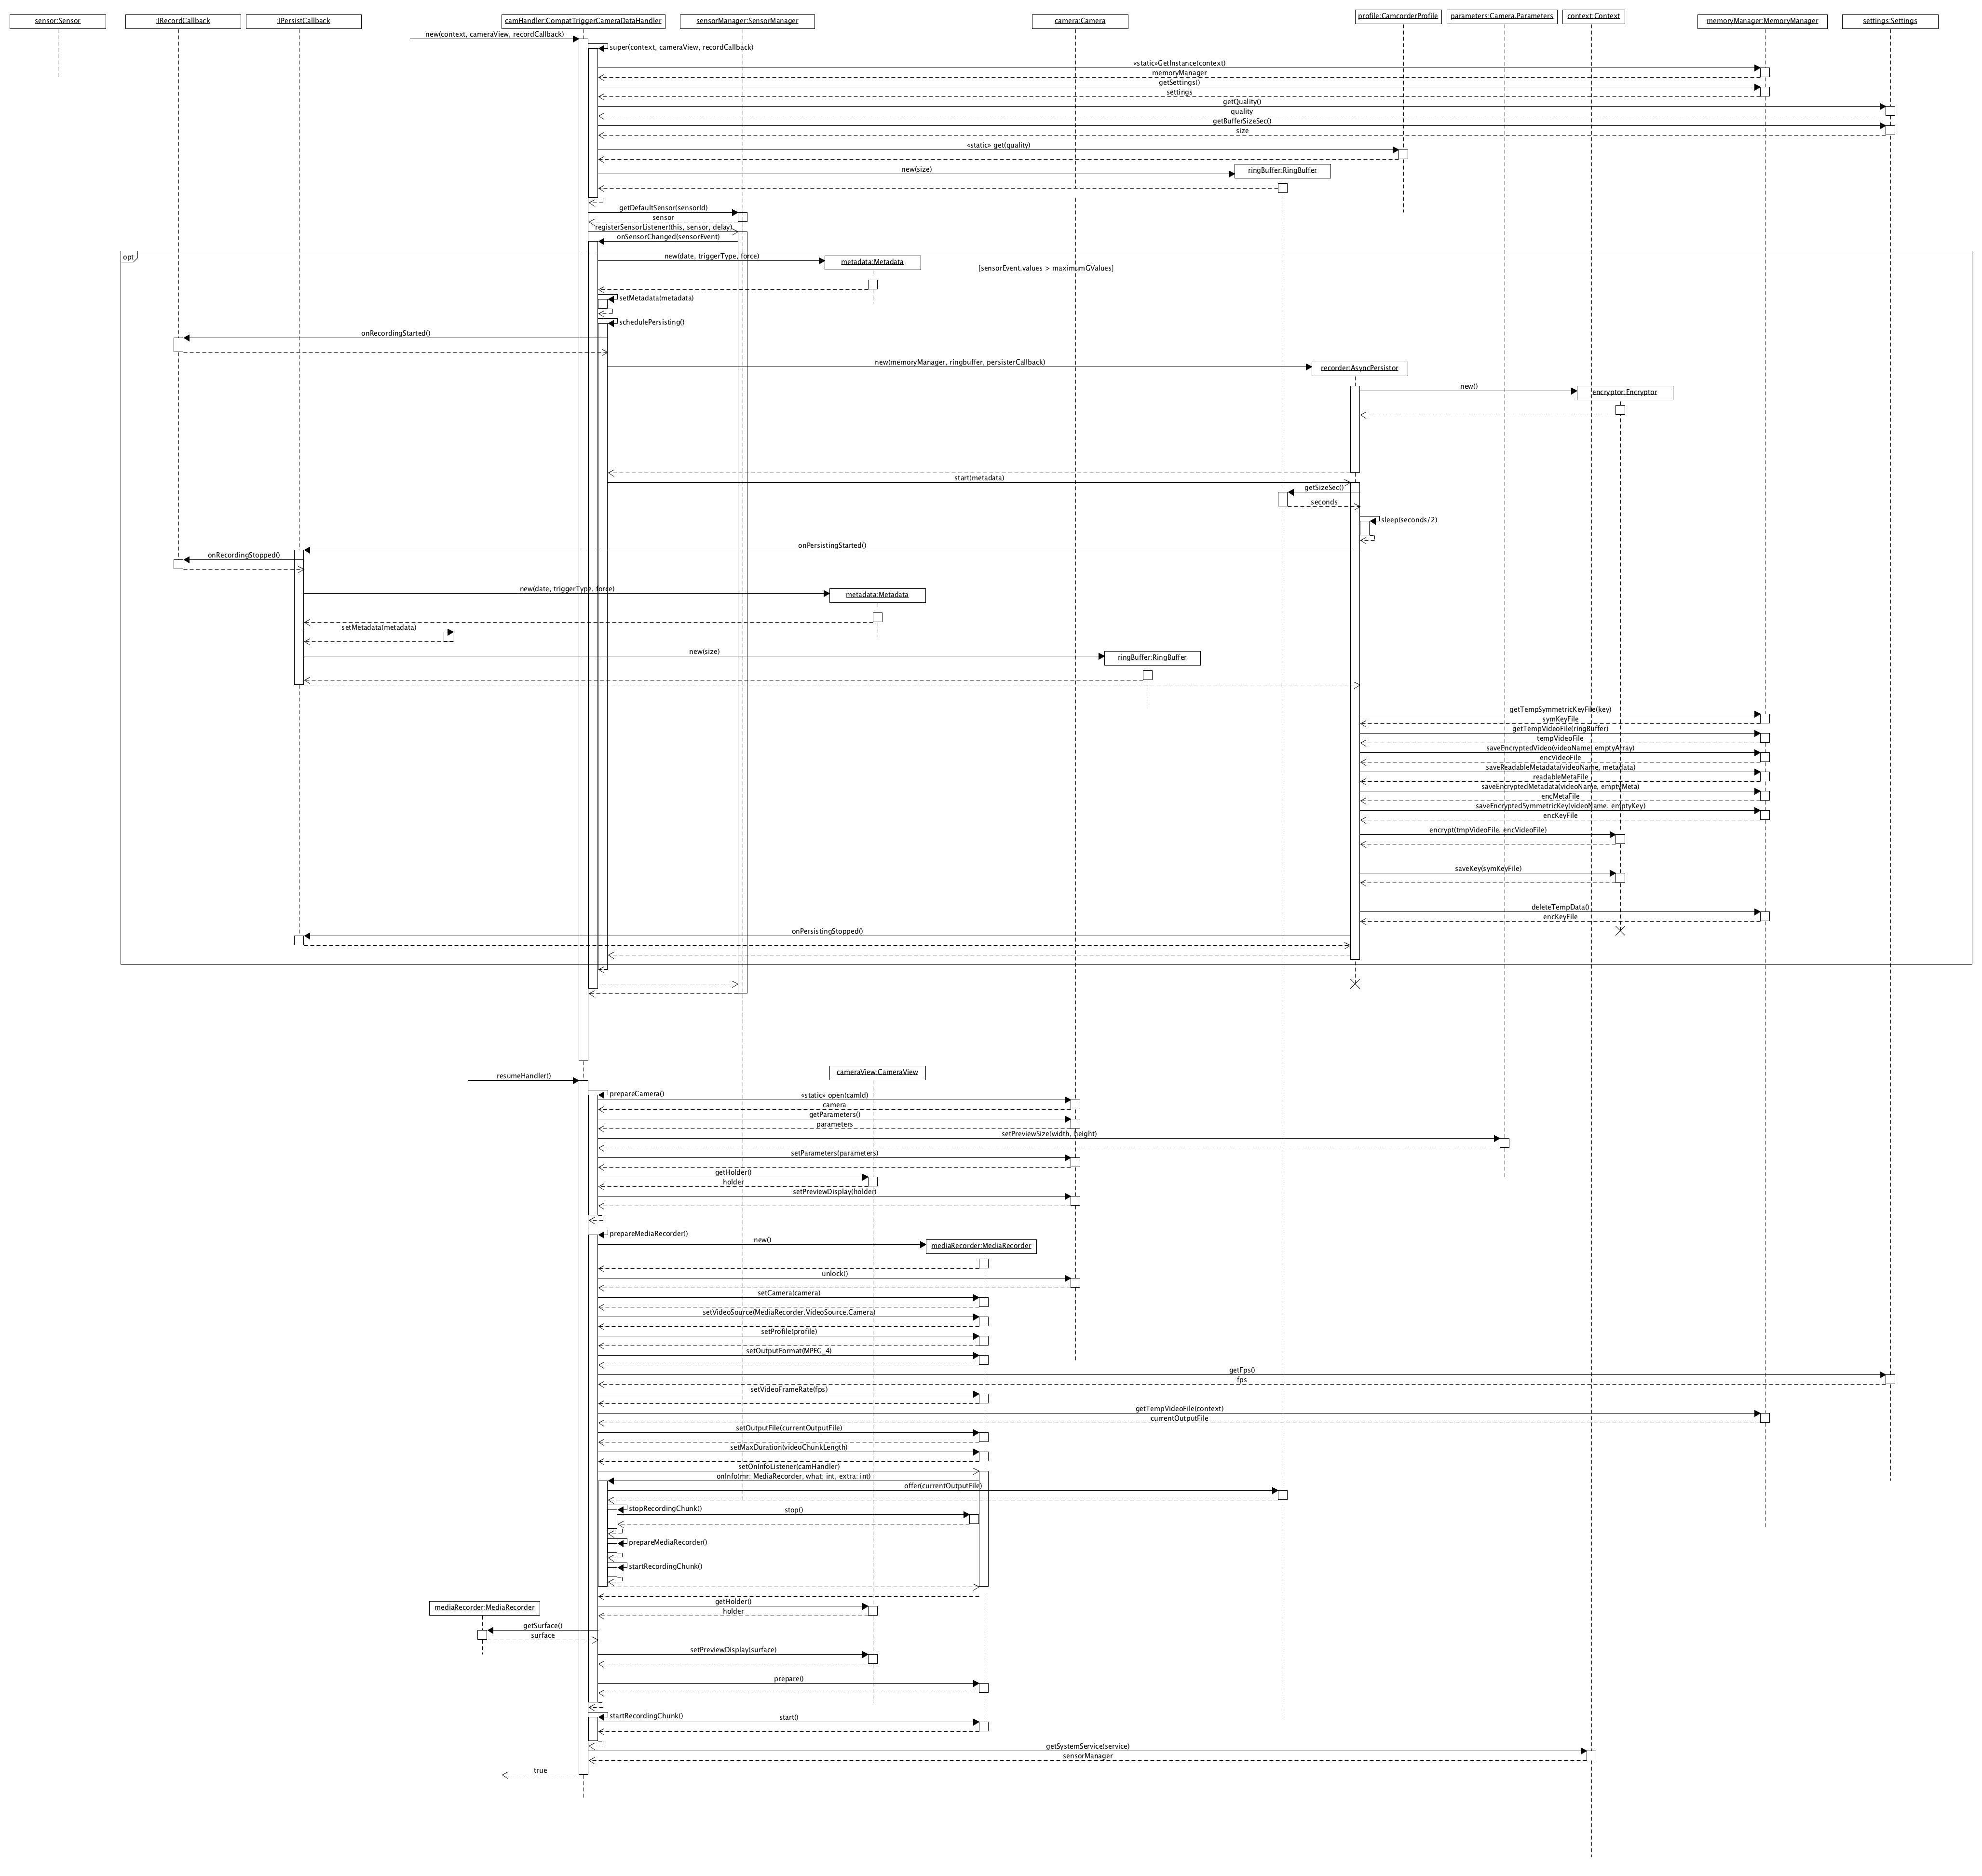
\includegraphics[width=1\textwidth]{./resources/Diagramme/App/recordSequence.jpg}
\caption{Videoaufnahme in der App}
	\label{fig:AppVideo}
\end{figure}

\begin{figure}[ht]
	\centering
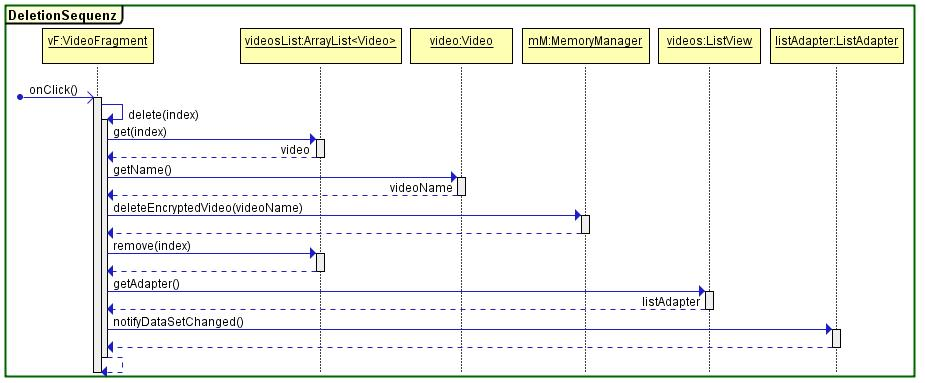
\includegraphics[width=1\textwidth]{./resources/Diagramme/App/deleteVideoSequence.jpg}
\caption{Video in der App löschen}
	\label{fig:AppDel}
\end{figure}

\begin{figure}[ht]
	\centering
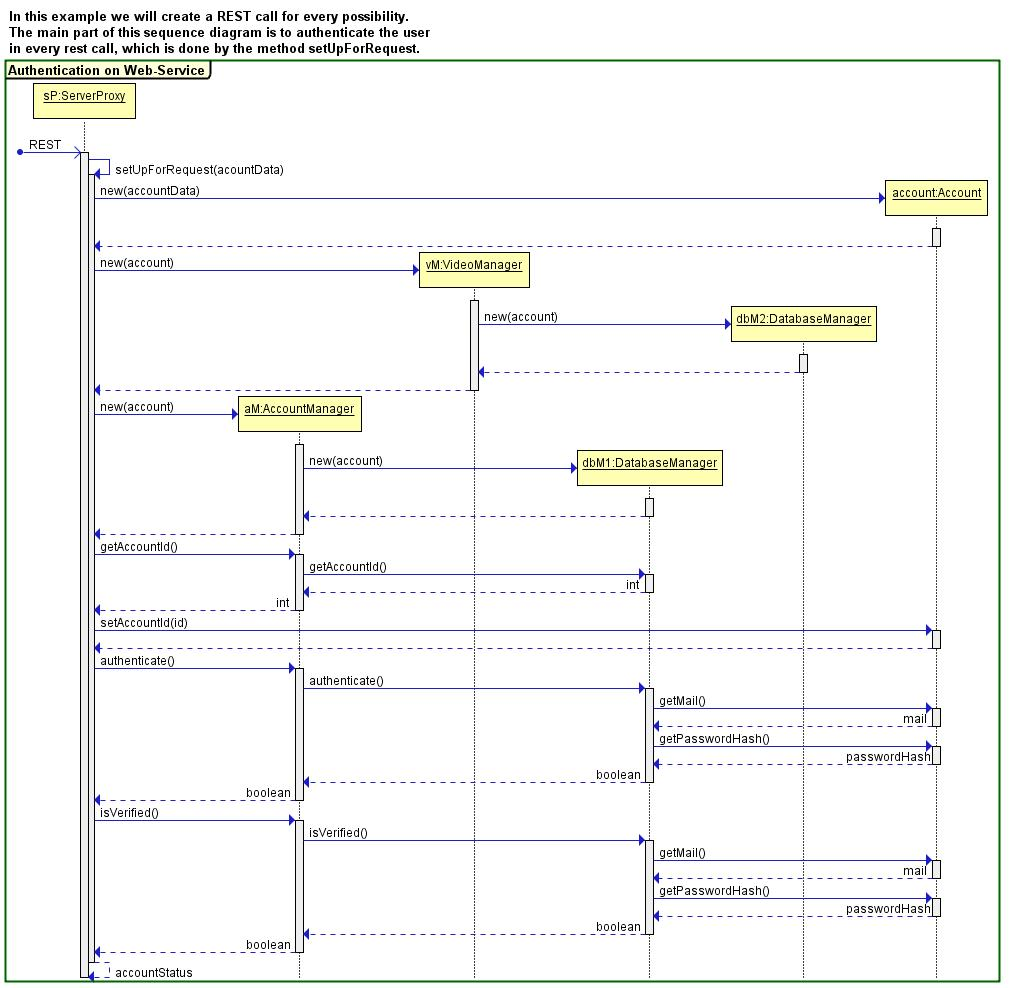
\includegraphics[width=1\textwidth]{./resources/Diagramme/Webservice/SeqAuthenticate.jpg}
\caption{Authentifizieren auf dem Dienst}
	\label{fig:ServiceAuth}
\end{figure}

\begin{figure}[ht]
	\centering
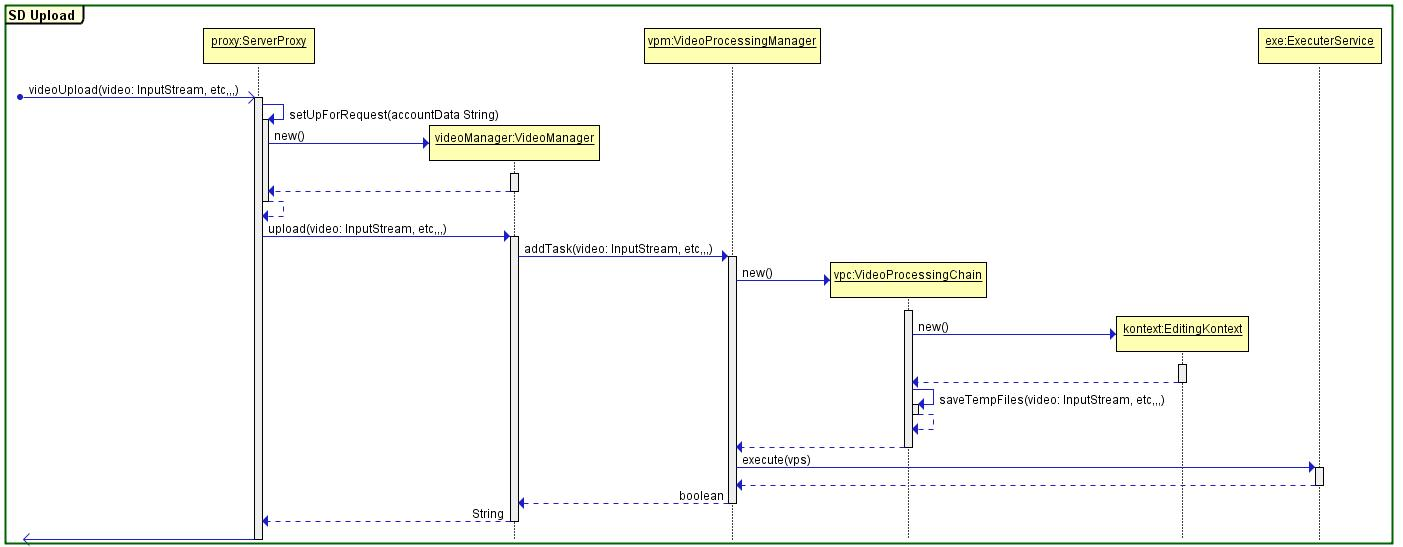
\includegraphics[width=1\textwidth]{./resources/Diagramme/Webservice/Upload.jpg}
\caption{Video auf den Dienst hochladen}
	\label{fig:ServiceUpload}
\end{figure}

\begin{figure}[ht]
	\centering
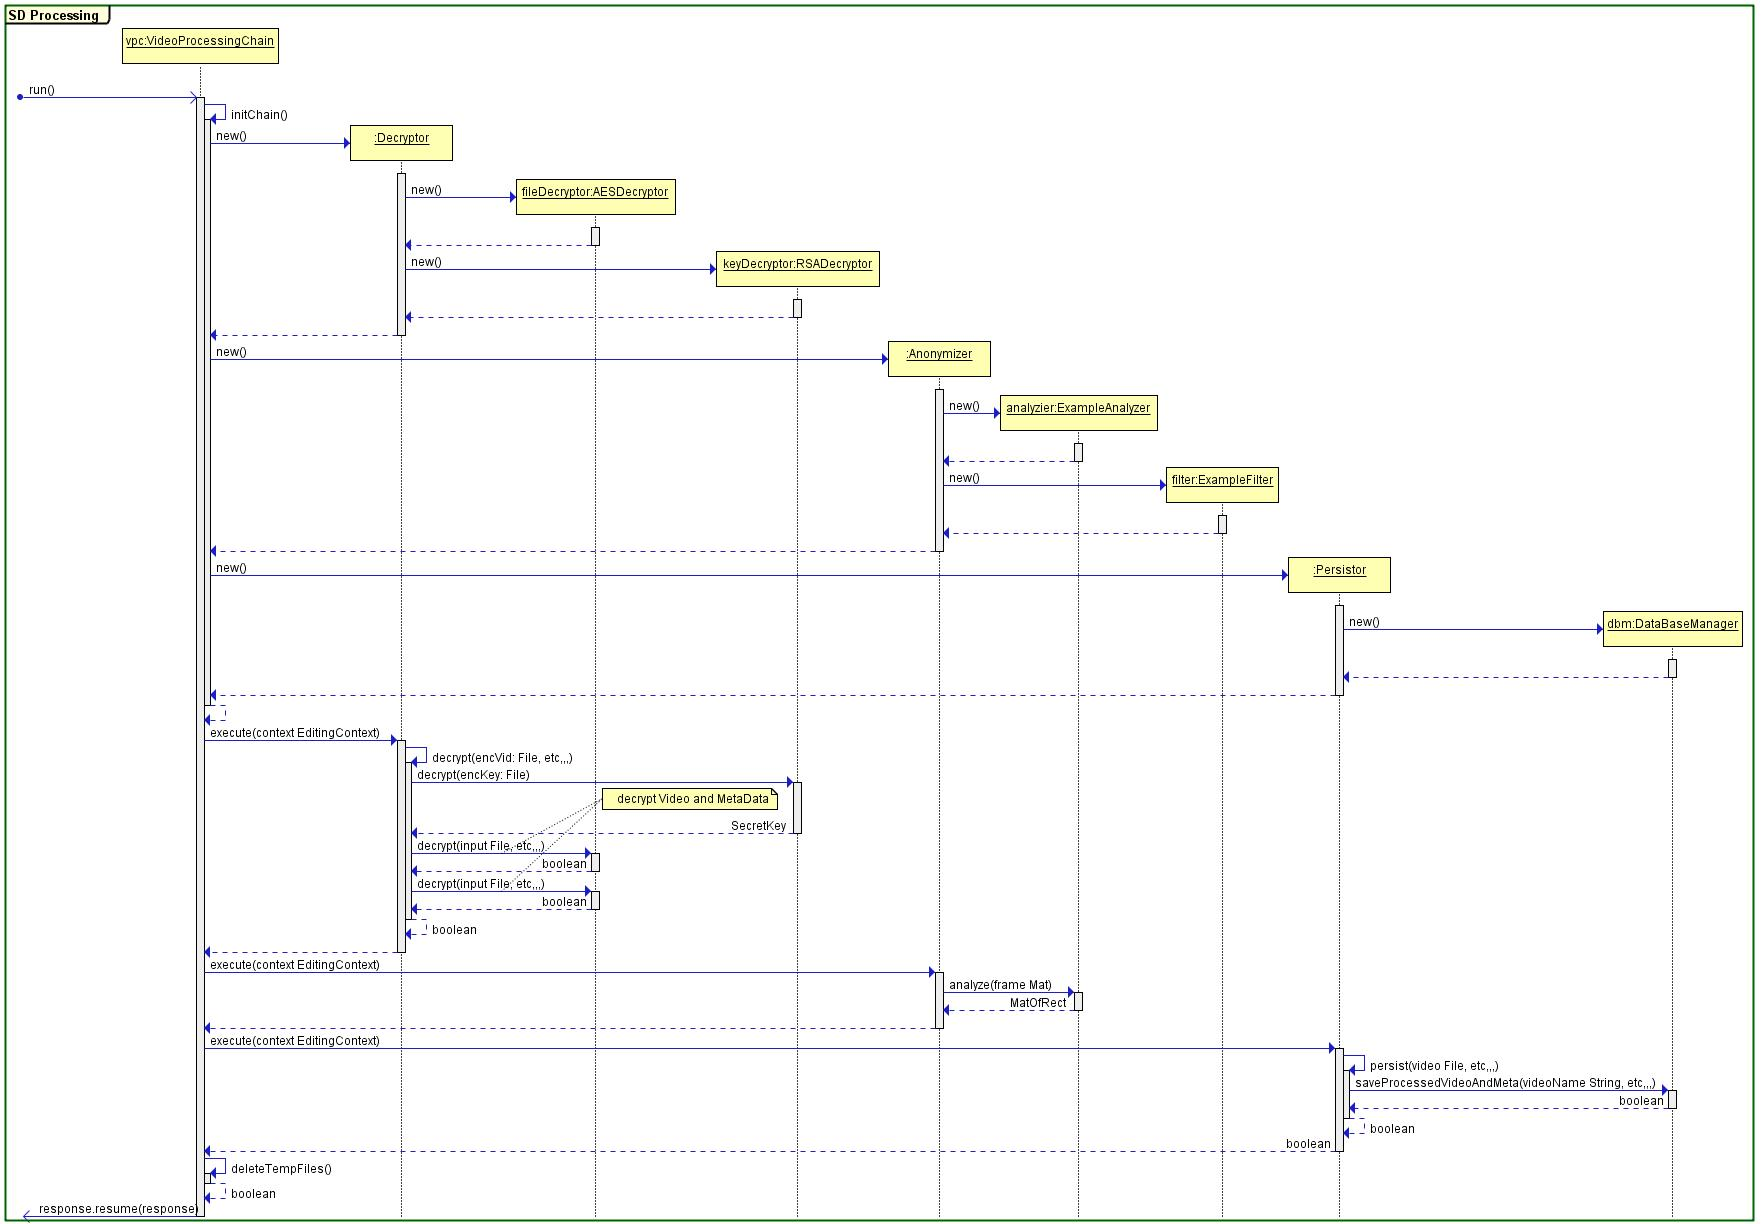
\includegraphics[width=1\textwidth]{./resources/Diagramme/Webservice/Processing.jpg}
\caption{Videobearbeitung auf dem Dienst}
	\label{fig:ServiceProcess}
\end{figure}

\begin{figure}[ht]
	\centering
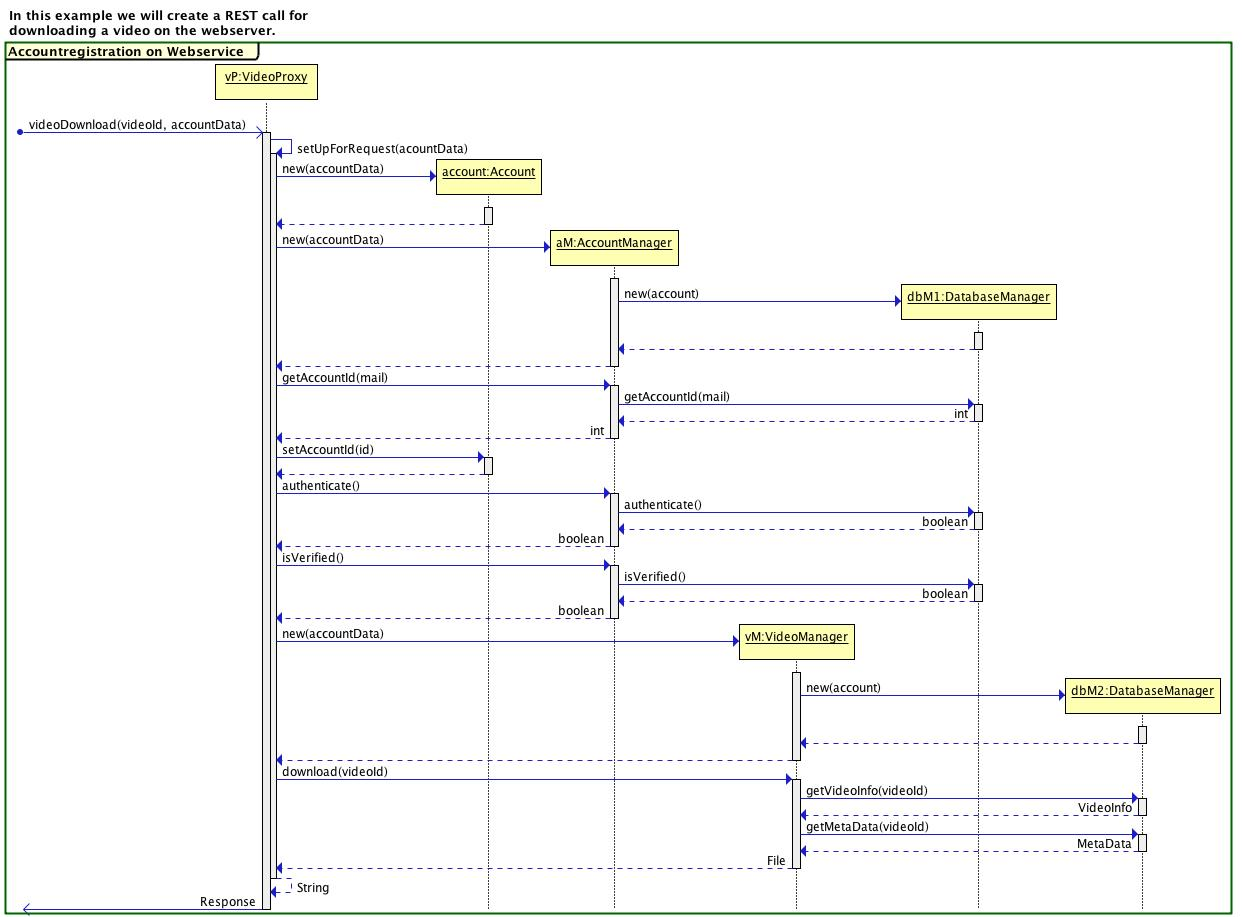
\includegraphics[width=1\textwidth]{./resources/Diagramme/Webservice/SeqVideoDownload.jpg}
\caption{Videodownload vom Dienst}
	\label{fig:ServiceDownl}
\end{figure}

\begin{figure}[ht]
	\centering
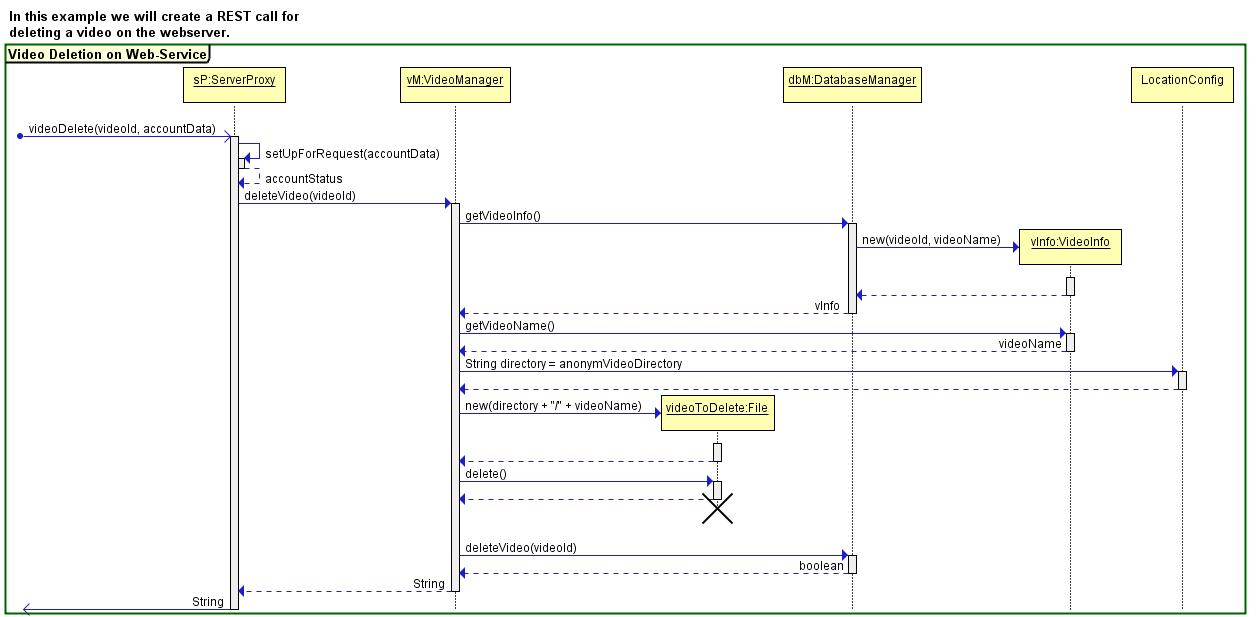
\includegraphics[width=1\textwidth]{./resources/Diagramme/Webservice/SeqVideoDeletion.jpg}
\caption{Video auf dem Dienst löschen}
	\label{fig:ServiceDel}
\end{figure}

%end content

\end{document}

